% !TeX program = xelatex
\documentclass[a4paper,10pt]{article}

% ============================================================================
% សន្លឹកកិច្ចការសិស្សបំពេញចន្លោះ ស-ខ្មៅ និងប្លង់ក្ដារខៀន/ចម្លើយគ្រូ (គ្មាន LCD / គ្មានកន្ត្រៃ)
% មេរៀនទី៤ (១)៖ ផ្ទៃក្រឡានិងមាឌ — ត្រូវគ្នា ១០០% នឹង LS_Plan_MEAS41.tex
% ============================================================================
\usepackage[a4paper, left=1.0cm, right=1.0cm, top=0.75cm, bottom=1.00cm, footskip=0.52cm]{geometry}
\usepackage{amsmath}
\usepackage{unicode-math}
\usepackage{fontspec}
\usepackage{array, colortbl}
\usepackage[table]{xcolor}
\usepackage{enumitem}
\usepackage{pifont}
\usepackage{fancyhdr}
\usepackage{lastpage}
\usepackage{tikz}
\usepackage[most]{tcolorbox}
\usetikzlibrary{calc, arrows.meta, decorations.pathreplacing, positioning, babel}

\makeatletter
\let\@expl@@@mark@update@singlecol@structures@@\relax
\makeatother

\providecommand{\NGSFindFonts}{%
  \IfFileExists{C:/Windows/Fonts/cambria.ttc}{%
    \def\NGSSysPath{C:/Windows/Fonts/}%
    \def\NGSUserPath{C:/Users/KIT/AppData/Local/Microsoft/Windows/Fonts/}%
  }{%
    \IfFileExists{./fonts/KhmerOSsiemreap.ttf}{\def\NGSSysPath{./fonts/}\def\NGSUserPath{./fonts/}}{%
    \IfFileExists{../fonts/KhmerOSsiemreap.ttf}{\def\NGSSysPath{../fonts/}\def\NGSUserPath{../fonts/}}{%
    \IfFileExists{../../fonts/KhmerOSsiemreap.ttf}{\def\NGSSysPath{../../fonts/}\def\NGSUserPath{../../fonts/}}{%
    \IfFileExists{../../../fonts/KhmerOSsiemreap.ttf}{\def\NGSSysPath{../../../fonts/}\def\NGSUserPath{../../../fonts/}}{%
    \IfFileExists{../../../../fonts/KhmerOSsiemreap.ttf}{\def\NGSSysPath{../../../../fonts/}\def\NGSUserPath{../../../../fonts/}}{%
    \IfFileExists{../../../../../fonts/KhmerOSsiemreap.ttf}{\def\NGSSysPath{../../../../../fonts/}\def\NGSUserPath{../../../../../fonts/}}{%
    \IfFileExists{../../../../../../fonts/KhmerOSsiemreap.ttf}{\def\NGSSysPath{../../../../../../fonts/}\def\NGSUserPath{../../../../../../fonts/}}{%
      \def\NGSSysPath{../../../../../../../fonts/}\def\NGSUserPath{../../../../../../../fonts/}%
    }}}}}}}%
  }%
}
\NGSFindFonts

\setmathfont[Path={\NGSSysPath}, FontIndex=1, Scale=1.02]{cambria.ttc}
\defaultfontfeatures{Ligatures=TeX}

\setmainfont[
  Path={\NGSUserPath}, Extension=.ttf, Script=Khmer,
  BoldFont={KhmerOSsiemreap}, BoldFeatures={FakeBold=1.8},
  ItalicFont={KhmerOSsiemreap}, ItalicFeatures={FakeSlant=0.25},
  BoldItalicFont={KhmerOSsiemreap}, BoldItalicFeatures={FakeBold=1.8, FakeSlant=0.25}
]{KhmerOSsiemreap}

\newfontfamily\muol[Path={\NGSUserPath}, Extension=.ttf, Script=Khmer]{KhmerOSmuollight}
\newfontfamily\TimesEn[Path={\NGSSysPath}, Extension=.ttf, BoldFont={timesbd}, ItalicFont={timesi}, BoldItalicFont={timesbi}]{times}
\newfontfamily\CalibriFont[Path={\NGSSysPath}, Extension=.ttf]{calibri}

\XeTeXlinebreaklocale "km"
\XeTeXlinebreakskip = 0pt plus 1pt minus 0.1pt

\definecolor{panelgray}{gray}{0.94}
\definecolor{headgray}{gray}{0.85}

\pagestyle{fancy}
\fancyhf{}
\renewcommand{\headrulewidth}{0pt}
\fancyfoot[L]{\fontsize{7.4pt}{9.5pt}\selectfont អនុវិទ្យាល័យព្រះក្រសាំង \en{|} គ្រូ៖ ហុក ប៊ុនថែន \en{|} មេរៀនទី៤ (១) ផ្ទៃក្រឡានិងមាឌ \en{|} ថ្ងៃចន្ទ ទី៣០ ខែវិច្ឆិកា ឆ្នាំ២០២៦}
\fancyfoot[R]{\fontsize{7.8pt}{10pt}\selectfont ទំព័រ \en{\thepage\ / \pageref{LastPage}}}

\setlength{\parindent}{0pt}
\setlength{\parskip}{0pt}
\setlength{\tabcolsep}{4pt}

\newcommand{\en}[1]{{\TimesEn #1}}
\newcommand{\enbf}[1]{{\TimesEn\bfseries #1}}
\newcommand{\unit}[1]{\,\text{\en{#1}}}
\newcommand{\riel}{\,\text{៛}}
\newcommand{\cnum}[1]{\mbox{\fontsize{10pt}{12pt}\selectfont\ding{\numexpr181+#1\relax}}}
\newcommand{\chkbox}{\tikz[baseline=-0.15ex]\draw[black, line width=0.85pt, fill=white] (0,0) rectangle (0.24cm,0.24cm);}
\newcommand{\ansbox}[1][1.75cm]{\,\tikz[baseline=-0.65ex]\draw[black, line width=0.65pt, fill=white] (0,0) rectangle (#1, 0.42cm);\,}
\newcommand{\dotline}[1][2.2cm]{\makebox[#1]{\dotfill}}

\newcommand{\pagebanner}[2]{%
  \begin{tcolorbox}[
    enhanced, sharp corners, colback=headgray, colframe=black,
    boxrule=1.05pt, boxsep=1pt, top=2.5pt, bottom=2.5pt, left=6pt, right=6pt,
    after skip=3.5pt
  ]
    {\muol\fontsize{9.0pt}{13.2pt}\selectfont #1}\hfill{\fontsize{8.0pt}{11.2pt}\selectfont\textbf{#2}}
  \end{tcolorbox}%
}

\newcommand{\secstrip}[2]{%
  \vspace{3pt}%
  \begin{tcolorbox}[
    enhanced, sharp corners, colback=panelgray, colframe=black,
    boxrule=0.8pt, boxsep=0.8pt, top=2pt, bottom=2pt, left=5pt, right=5pt,
    after skip=3pt
  ]
    {\muol\fontsize{8.5pt}{12.2pt}\selectfont #1}\hfill{\fontsize{7.8pt}{10.8pt}\selectfont\textit{#2}}
  \end{tcolorbox}%
}

\newcolumntype{L}[1]{>{\raggedright\arraybackslash}p{#1}}
\newcolumntype{C}[1]{>{\centering\arraybackslash}p{#1}}

\begin{document}
\fontsize{9.5pt}{14.5pt}\selectfont

% ============================================================================
% ទំព័រទី ១៖ សន្លឹកកិច្ចការសិស្ស (ផ្នែកមុខ៖ E1 -> E2 -> E3)
% ============================================================================
\pagebanner{សន្លឹកកិច្ចការសិស្ស \enbf{(}៤\enbf{.}១ ផ្ទៃក្រឡានិងមាឌ\enbf{)} \enbf{--} ផ្នែកមុខ}{ថ្នាក់ទី៨ \en{|} សៀវភៅគោល ទំ.៤៣--៤៤}

\begin{tcolorbox}[
  enhanced, sharp corners, colback=white, colframe=black,
  boxrule=0.8pt, boxsep=1.5pt, top=3.5pt, bottom=3.5pt, left=5pt, right=5pt,
  after skip=4pt
]
  \fontsize{9.0pt}{13.0pt}\selectfont
  \textbf{ឈ្មោះសិស្ស៖} \dotline[4.3cm] \quad
  \textbf{សមាជិកក្រុម៖} \dotline[4.3cm] \quad
  \textbf{ថ្នាក់ទី៖} ៨\dotline[0.9cm] \quad
  \textbf{ក្រុមទី៖} \dotline[1.0cm]
\end{tcolorbox}

% --- E1 Engage ---
\secstrip{ផ្នែកទី ១ \enbf{(E1 - Engage)} ៖ បេសកកម្មជាងអគ្គិសនីវាស់បន្ទះការេតូចជ្រុង $1\unit{mm}$}{រយៈពេល ៣ នាទី (គូស \ding{51} ក្នុង \chkbox)}

\begin{tcolorbox}[
  enhanced, sharp corners, colback=white, colframe=black,
  boxrule=0.8pt, boxsep=2pt, top=3.5pt, bottom=3.5pt, left=6pt, right=6pt
]
  ជាងអគ្គិសនីម្នាក់វាស់ឃើញបន្ទះលោហៈរាងការេតូចមួយមានជ្រុង $a = 1\unit{mm} = 0.001\unit{m} = 10^{-3}\unit{m}$ ៖\\[2pt]
  $\bullet$ \textbf{តើកូនជាងរូបណាបំប្លែងផ្ទៃក្រឡាជា $\unit{m}^2$ បានត្រឹមត្រូវ?} \quad
  \chkbox\ \textbf{កូនជាងទី ១៖} $S = 10^{-3}\unit{m}^2$ \qquad
  \chkbox\ \textbf{កូនជាងទី ២៖} $S = 10^{-6}\unit{m}^2$\\[2pt]
  $\bullet$ \textbf{ហេតុផលខ្លី៖} បើជ្រុង $a = 10^{-3}\unit{m}$ នោះផ្ទៃក្រឡាការេ $S = a\times a =$ \dotline[6.4cm] ។
\end{tcolorbox}

\vfill

% --- E2 Explore ---
\secstrip{ផ្នែកទី ២ \enbf{(E2 - Explore)} ៖ ការបំប្លែងខ្នាតតូច និងផ្ទៃមុខកាត់ខ្សែភ្លើង (ទំ.៤៣--៤៤)}{រយៈពេល ១១ នាទី}

\textbf{សកម្មភាព ១ (\en{E2-A} — ៦ នាទី)៖ តារាងបំប្លែងខ្នាតស្វ័យគុណគោល $10$ និងលំហាត់គំរូទី ១ ($d = 2\unit{mm}, \pi = 3.14$)}

\begin{tcolorbox}[
  enhanced, sharp corners, colback=white, colframe=black,
  boxrule=0.8pt, boxsep=2pt, top=3.5pt, bottom=3.5pt, left=6pt, right=6pt
]
  $\bullet$ \textbf{បំប្លែងប្រវែងជាម៉ែត្រ (ទំ.៤៣)៖} $1\unit{mm} = 0.001\unit{m} =$ \ansbox[1.4cm] $\unit{m}$; \quad
  $1\unit{cm} = 0.01\unit{m} =$ \ansbox[1.4cm] $\unit{m}$; \quad $1\unit{dm} = 0.1\unit{m} =$ \ansbox[1.4cm] $\unit{m}$\\[3pt]
  $\bullet$ \textbf{លំហាត់គំរូទី ១ (ទំ.៤៣--៤៤)៖} ខ្សែភ្លើងរាងស៊ីឡាំងមានអង្កត់ផ្ចិត $d = 2\unit{mm}$ ។ រកផ្ទៃក្រឡាមុខកាត់ $S$ គិតជា $\unit{m}^2$ ($\pi = 3.14$) ៖\\[2pt]
  \hspace*{0.3cm}-- ជំហាន \cnum{1} បំប្លែងអង្កត់ផ្ចិត៖ $d = 2\unit{mm} = 2 \times$ \dotline[1.4cm] $\unit{m} \implies d^2 = (2\times 10^{-3}\unit{m})^2 =$ \ansbox[2.2cm] $\unit{m}^2$\\[3pt]
  \hspace*{0.3cm}-- ជំហាន \cnum{2} ផ្ទៃមុខកាត់រង្វង់៖ $S = \pi\times \dfrac{d^2}{4} = 3.14 \times \dfrac{\dotline[2.0cm]}{4} =$ \dotline[2.2cm] $\unit{m}^2 =$ \ansbox[2.3cm] $\unit{m}^2$ ($314\times 10^{-8}\unit{m}^2$)
\end{tcolorbox}

\vspace{3pt}
\textbf{សកម្មភាព ២ (\en{E2-B} — ៥ នាទី)៖ ពិនិត្យអន្ទាក់ភ្លេចលើកការេខ្នាត និងអន្ទាក់ភ្លេចចែកនឹង $4$}

\begin{tcolorbox}[
  enhanced, sharp corners, colback=white, colframe=black,
  boxrule=0.8pt, boxsep=2pt, top=3.5pt, bottom=3.5pt, left=6pt, right=6pt
]
  $\bullet$ \textbf{អន្ទាក់ទី ១ (ខ្នាតផ្ទៃក្រឡា និងមាឌ)៖} ដោយសារ $1\unit{cm} = 10^{-2}\unit{m}$ នោះ $1\unit{cm}^2 = (10^{-2}\unit{m})^2 =$ \dotline[1.6cm] $\unit{m}^2$ ហើយ $1\unit{cm}^3 = (10^{-2}\unit{m})^3 =$ \dotline[1.6cm] $\unit{m}^3$ ។\\[3pt]
  $\bullet$ \textbf{អន្ទាក់ទី ២ (អង្កត់ផ្ចិត $d$ ទល់នឹងកាំ $r$)៖} កាំរង្វង់ $r = \dfrac{d}{2} \implies r^2 = \dfrac{d^2}{\dotline[0.8cm]}$ ។ បើភ្លេចចែកនឹង $4$ ចម្លើយនឹងធំជាងការពិត \dotline[1.0cm] ដង!
\end{tcolorbox}

\vfill

% --- E3 Explain ---
\secstrip{ផ្នែកទី ៣ \enbf{(E3 - Explain)} ៖ រូបមន្តផ្ទៃក្រឡា-មាឌវិមាត្រតូច និងធនាគារហេតុផល \enbf{B\&W}}{រយៈពេល ៦ នាទី}

\begin{tcolorbox}[
  enhanced, sharp corners, colback=white, colframe=black,
  boxrule=0.85pt, boxsep=2pt, top=3.5pt, bottom=3.5pt, left=6pt, right=6pt
]
  ១) \textbf{មុខកាត់រាងរង្វង់ស្គាល់ $d$៖} $S = \pi\times \dfrac{d^2}{\dotline[0.9cm]}$ \qquad
  ២) \textbf{ទាញរកអង្កត់ផ្ចិត $d$៖} $d = \sqrt{\dfrac{4\times \dotline[0.9cm]}{\pi}}$ \qquad
  ៣) \textbf{មាឌស៊ីឡាំង៖} $V = S\times l = \dfrac{\pi d^2}{4}\times \dotline[0.9cm]$\\[4pt]
  \tikz\draw[black, dashed, line width=0.5pt] (0,0) -- (18.4cm,0);\\[3pt]
  \fontsize{8.8pt}{12.8pt}\selectfont
  \textbf{ធនាគារហេតុផល (\en{Warrant Bank})៖} \quad
  \cnum{1} \textbf{បំប្លែងជា $\unit{m}$ មុន៖} $1\unit{mm}=10^{-3}\unit{m} \implies 1\unit{mm}^2=10^{-6}\unit{m}^2$; \ $1\unit{cm}=10^{-2}\unit{m} \implies 1\unit{cm}^2=10^{-4}\unit{m}^2$\\
  \cnum{2} \textbf{មុខកាត់រង្វង់៖} $S = \frac{\pi d^2}{4}$ \quad
  \cnum{3} \textbf{រកអង្កត់ផ្ចិត៖} $d = \sqrt{\frac{4S}{\pi}}$ \quad
  \cnum{4} \textbf{មាឌវត្ថុមុខកាត់ស្មើ៖} $V = S\times l$ (ឈើជ្រុង $V = a\times b\times l$ គិតជា $\unit{m}^3$)
\end{tcolorbox}

% ============================================================================
% ទំព័រទី ២៖ សន្លឹកកិច្ចការសិស្ស (ផ្នែកខាងខ្នង៖ E4 -> E5 -> កិច្ចការផ្ទះ)
% ============================================================================
\clearpage
\pagebanner{សន្លឹកកិច្ចការសិស្ស \enbf{(}៤\enbf{.}១ ផ្ទៃក្រឡានិងមាឌ\enbf{)} \enbf{--} ផ្នែកខាងខ្នង}{ថ្នាក់ទី៨ \en{|} សៀវភៅគោល ទំ.៤៤, ៥០}

% --- E4 Elaborate ---
\secstrip{ផ្នែកទី ៤ \enbf{(E4 - Elaborate)} ៖ លំហាត់គំរូទី ២ — គណនាអង្កត់ផ្ចិតខ្សែភ្លើង (ទំ.៤៤)}{រយៈពេល ១០ នាទី}

\begin{tcolorbox}[
  enhanced, sharp corners, colback=white, colframe=black,
  boxrule=0.8pt, boxsep=2pt, top=3.5pt, bottom=3.5pt, left=6pt, right=6pt
]
  \textbf{១) លំហាត់គំរូទី ២ (ទំ.៤៤)៖} គណនាអង្កត់ផ្ចិតខ្សែភ្លើង $d$ (គិតជា $\unit{m}$) ដោយដឹងថាវាមានផ្ទៃក្រឡាមុខកាត់ស្មើនឹង $S = \dfrac{\pi}{4}\times 10^{-6}\unit{m}^2$ ៖\\[3pt]
  $\bullet$ \textbf{ជំហានទី ១ (ទាញរូបមន្ត \cnum{3})៖} ពី $S = \dfrac{\pi\cdot d^2}{4} \implies d^2 = \dfrac{4S}{\pi} \implies d = \sqrt{\dfrac{\dotline[1.4cm]}{\pi}}$\\[3pt]
  $\bullet$ \textbf{ជំហានទី ២ (ជំនួសតម្លៃ $S$)៖} $d = \sqrt{\dfrac{4}{\pi}\times \dfrac{\pi\times 10^{-6}}{4}} = \sqrt{\dotline[1.5cm]} =$ \ansbox[2.0cm] $\unit{m}$ ($=$ \dotline[1.2cm] $\unit{mm}$)\\[3pt]
  \textbf{២) អនុវត្តភ្ជាប់ឈើជ្រុង (\cnum{4})៖} ឈើជ្រុង ១ ដើម មានមុខកាត់ $4\unit{cm}\times 8\unit{cm}$ និងប្រវែង $l = 5\unit{m}$៖
  បំប្លែង $4\unit{cm} = 0.04\unit{m}, \ 8\unit{cm} = 0.08\unit{m} \implies V =$ \ansbox[2.1cm] $\unit{m}^3$\\[2pt]
  \fontsize{8.7pt}{12.5pt}\selectfont
  \textbf{ឆ្លុះបញ្ចាំង (\en{EIA Looking-Back})៖} បើអង្កត់ផ្ចិតខ្សែភ្លើងកើន $2$ ដង នោះផ្ទៃក្រឡាមុខកាត់ $S$ កើនឡើង \dotline[1.2cm] ដង ។
\end{tcolorbox}

\vfill

% --- E5 Evaluate ---
\secstrip{ផ្នែកទី ៥ \enbf{(E5 - Evaluate)} ៖ លំហាត់ប្រតិបត្តិ (ទំ.៤៤) សំណួរវិនិច្ឆ័យ \enbf{A--D} និងសំបុត្រចេញ}{រយៈពេល ១០ នាទី}

\begin{tcolorbox}[
  enhanced, sharp corners, colback=white, colframe=black,
  boxrule=0.8pt, boxsep=2pt, top=3.5pt, bottom=3.5pt, left=6pt, right=6pt
]
  \textbf{១) ប្រតិបត្តិ (ទំ.៤៤)៖} គណនាមាឌរបស់ខ្សែភ្លើងដែលមានអង្កត់ផ្ចិត $d = 2\unit{cm}$ ហើយមានប្រវែង $l = 200\unit{m}$ ($\pi = 3.14$) ៖\\[3pt]
  $\bullet$ បំប្លែងអង្កត់ផ្ចិត (\cnum{1})៖ $d = 2\unit{cm} = 2\times$ \dotline[1.4cm] $\unit{m} \implies d^2 =$ \dotline[2.0cm] $\unit{m}^2$\\[3pt]
  $\bullet$ ផ្ទៃក្រឡាមុខកាត់ (\cnum{2})៖ $S = 3.14\times \dfrac{d^2}{4} =$ \dotline[2.3cm] $\unit{m}^2$\\[3pt]
  $\bullet$ មាឌខ្សែភ្លើង (\cnum{4})៖ $V = S\times l =$ \dotline[2.2cm] $\times 200 =$ \ansbox[2.5cm] $\unit{m}^3$ ($=$ \dotline[1.8cm] $\unit{m}^3$)\\[3pt]
  \textbf{២) បិទបេសកកម្ម \en{E1} (ការេជ្រុង $1\unit{mm} = 10^{-3}\unit{m}$)៖} កូនជាងទី \dotline[0.9cm] ត្រឹមត្រូវ ព្រោះ $S = (10^{-3}\unit{m})^2 =$ \dotline[1.8cm] $\unit{m}^2$ ។
\end{tcolorbox}

\vspace{3.5pt}

\begin{tcolorbox}[
  enhanced, sharp corners, colback=white, colframe=black,
  boxrule=0.8pt, boxsep=2pt, top=3.5pt, bottom=3.5pt, left=6pt, right=6pt
]
  \textbf{៣) សំណួរវិនិច្ឆ័យ \en{A--D} (សរសៃដែកសាងសង់អង្កត់ផ្ចិត $d = 10\unit{mm}, \pi = 3.14$ តើផ្ទៃក្រឡាមុខកាត់ស្មើប៉ុន្មាន $\unit{m}^2$? — លើកម្រាមដៃ ១--៤)៖}\\[2.5pt]
  \textbf{\en{A.}} $314\times 10^{-6}\unit{m}^2$ \qquad
  \textbf{\en{B.}} $78.5\times 10^{-6}\unit{m}^2$ \qquad
  \textbf{\en{C.}} $78.5\times 10^{-3}\unit{m}^2$ \qquad
  \textbf{\en{D.}} $31.4\times 10^{-3}\unit{m}^2$\\[3.5pt]
  \tikz\draw[black, dashed, line width=0.5pt] (0,0) -- (18.4cm,0);\\[3pt]
  \textbf{៤) សំបុត្រចេញ ៦០ វិនាទី៖} ខ្សែភ្លើងអង្កត់ផ្ចិត $d = 4\unit{mm} = 4\times 10^{-3}\unit{m}$ និងប្រវែង $l = 100\unit{m}$ ($\pi = 3.14$)៖
  $S =$ \dotline[2.3cm] $\unit{m}^2$, \quad $V =$ \dotline[2.3cm] $\unit{m}^3$ ។
\end{tcolorbox}

\vfill

% --- Homework ---
\begin{tcolorbox}[
  enhanced, sharp corners, colback=panelgray, colframe=black,
  boxrule=0.95pt, boxsep=2pt, top=3.5pt, bottom=3.5pt, left=6pt, right=6pt
]
  {\muol\fontsize{9.0pt}{13.0pt}\selectfont កិច្ចការផ្ទះ \enbf{(}សៀវភៅគោល ទំ.៥០ លេខ ១ ក,ខ,គ, លេខ ២ ក និងលេខ ៣\enbf{)}}\\[2.5pt]
  \fontsize{8.8pt}{13.0pt}\selectfont
  $\bullet$ \textbf{\#1 (ក,ខ,គ — ទំ.៥០)៖} គណនាផ្ទៃក្រឡាមុខកាត់ស៊ីឡាំងគិតជា $\unit{m}^2$ ($\pi=3.14$) បើអង្កត់ផ្ចិតស្មើ៖ \textbf{ក.} $1.5\unit{mm}$ \quad \textbf{ខ.} $2.5\unit{mm}$ \quad \textbf{គ.} $0.2\unit{mm}$ ។\\
  $\bullet$ \textbf{\#2 (ក — ទំ.៥០)៖} គណនាមាឌសរសៃដែកដែលមានអង្កត់ផ្ចិត $d = 6\unit{mm}$ និងប្រវែង $l = 12\unit{m}$ ។\\
  $\bullet$ \textbf{\#3 (ទំ.៥០)៖} ឈើជ្រុងមួយដើមមានមុខកាត់ $4\unit{cm}\times 8\unit{cm}$ និងប្រវែង $4.5\unit{m}$ ។ បើទិញ $50$ ដើម តើត្រូវចំណាយប្រាក់អស់ប៉ុន្មាន បើឈើ $1\unit{m}^3$ ថ្លៃ $1\,200\,000\riel$? \textbf{អានមុន៖} ២. ម៉ាសធៀបនឹងផ្ទៃក្រឡា (ទំ.៤៤--៤៦) ។
\end{tcolorbox}

% ============================================================================
% ទំព័រទី ៣៖ ទំព័រគ្រូបង្រៀន (គំរូប្លង់ក្ដារខៀន ៣ ផ្នែក + ចម្លើយផ្ទៀងផ្ទាត់រហ័ស)
% ============================================================================
\clearpage
\pagebanner{ទំព័រគ្រូបង្រៀន ៖ ប្លង់ក្ដារខៀន \enbf{(}គ្មាន \enbf{LCD)} និងចម្លើយផ្ទៀងផ្ទាត់រហ័ស}{៤.១ ផ្ទៃក្រឡានិងមាឌ (\en{MEAS41})}

\secstrip{១. គំរូប្លង់បែងចែកក្ដារខៀន ៣ ផ្នែក សម្រាប់ថ្នាក់រៀនគ្មាន \enbf{LCD}}{សម្រាប់គ្រូប្រើដីស/ហ្វឺត}

\begin{center}
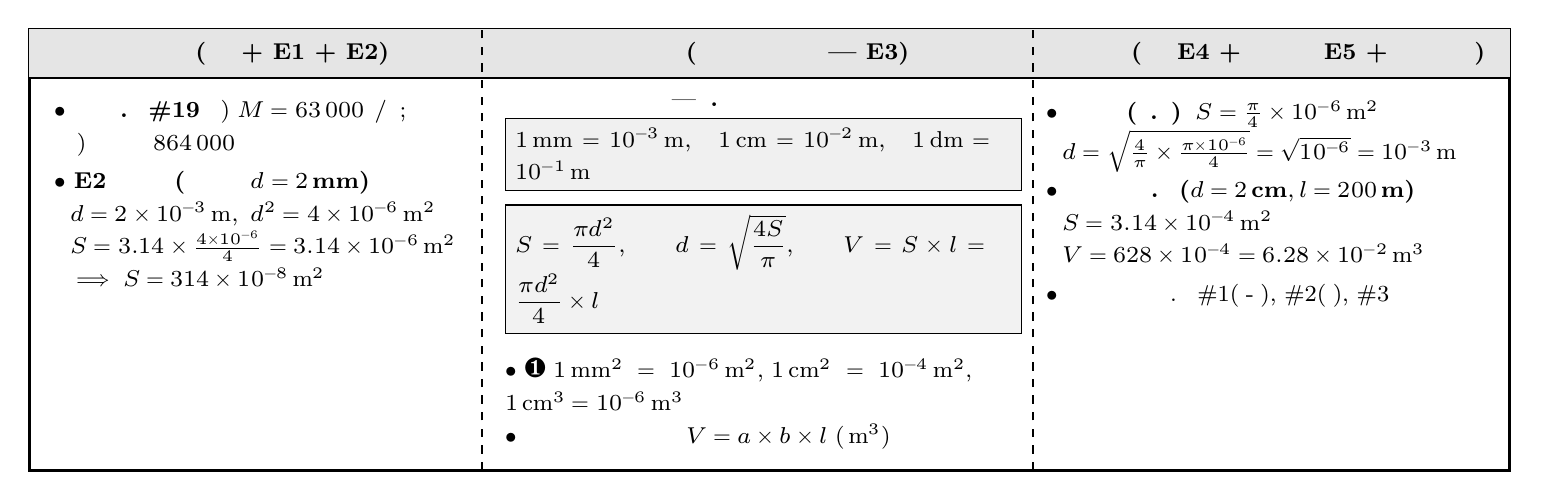
\begin{tikzpicture}[x=1cm, y=1cm, every node/.style={font=\fontsize{8.3pt}{11.8pt}\selectfont, text=black}]
  \draw[black, line width=1.1pt] (0,0) rectangle (18.8,5.60);
  \fill[gray!20] (0,4.98) rectangle (18.8,5.60);
  \draw[black, line width=0.7pt] (0,4.98) -- (18.8,4.98);
  \draw[black, dashed, line width=0.7pt] (5.75,0) -- (5.75,5.60);
  \draw[black, dashed, line width=0.7pt] (12.75,0) -- (12.75,5.60);

  \node at (2.875,5.29) {\textbf{ផ្នែកឆ្វេង (កំណែ + \en{E1} + \en{E2})}};
  \node at (9.25,5.29) {\textbf{ផ្នែកកណ្ដាល (ខ្លឹមសារគោលរក្សាទុក — \en{E3})}};
  \node at (15.775,5.29) {\textbf{ផ្នែកស្ដាំ (គំរូ \en{E4} + ប្រតិបត្តិ \en{E5} + កិច្ចការផ្ទះ)}};

  % Left
  \node[anchor=north west, text width=5.35cm] at (0.20,4.82) {%
    $\bullet$ \textbf{កំណែ ទំ.៤២ \#19៖} ក) $M=63\,000\riel$/ខែ;\\
    \hspace*{0.2cm}ខ) សន្សំបាន $864\,000\riel$\\[2pt]
    $\bullet$ \textbf{\en{E2} គំរូទី ១ (ខ្សែភ្លើង $d=2\unit{mm}$)៖}\\
    \hspace*{0.2cm}$d = 2\times 10^{-3}\unit{m}, \ d^2 = 4\times 10^{-6}\unit{m}^2$\\
    \hspace*{0.2cm}$S = 3.14\times \frac{4\times 10^{-6}}{4} = 3.14\times 10^{-6}\unit{m}^2$\\
    \hspace*{0.2cm}$\implies S = 314\times 10^{-8}\unit{m}^2$
  };

  % Center
  \node[anchor=north west, text width=6.65cm] at (5.92,4.82) {%
    {\muol\fontsize{8.5pt}{12pt}\selectfont មេរៀនទី៤៖ រង្វាស់រង្វាល់ — ១\enbf{.} ផ្ទៃក្រឡានិងមាឌ}\\[3pt]
    \tikz\node[draw=black, fill=gray!12, inner sep=3.5pt, text width=6.3cm]{%
      $1\unit{mm} = 10^{-3}\unit{m}, \quad 1\unit{cm} = 10^{-2}\unit{m}, \quad 1\unit{dm} = 10^{-1}\unit{m}$
    };\\[4pt]
    \tikz\node[draw=black, fill=gray!10, inner sep=3.5pt, text width=6.3cm]{%
      $S = \dfrac{\pi d^2}{4}, \qquad d = \sqrt{\dfrac{4S}{\pi}}, \qquad V = S\times l = \dfrac{\pi d^2}{4}\times l$
    };\\[4pt]
    $\bullet$ \cnum{1} $1\unit{mm}^2 = 10^{-6}\unit{m}^2$, $1\unit{cm}^2 = 10^{-4}\unit{m}^2$, $1\unit{cm}^3 = 10^{-6}\unit{m}^3$\\
    $\bullet$ ឈើជ្រុងមុខកាត់ចតុកោណកែង៖ $V = a\times b\times l$ ($\unit{m}^3$)
  };

  % Right
  \node[anchor=north west, text width=5.8cm] at (12.80,4.82) {%
    $\bullet$ \textbf{គំរូទី ២ (ទំ.៤៤)៖} $S = \frac{\pi}{4}\times 10^{-6}\unit{m}^2$\\
    \hspace*{0.2cm}$d = \sqrt{\frac{4}{\pi}\times \frac{\pi\times 10^{-6}}{4}} = \sqrt{10^{-6}} = 10^{-3}\unit{m}$\\[2pt]
    $\bullet$ \textbf{ប្រតិបត្តិ ទំ.៤៤ ($d=2\unit{cm}, l=200\unit{m}$)៖}\\
    \hspace*{0.2cm}$S = 3.14\times 10^{-4}\unit{m}^2$\\
    \hspace*{0.2cm}$V = 628\times 10^{-4} = 6.28\times 10^{-2}\unit{m}^3$\\[2pt]
    $\bullet$ \textbf{កិច្ចការផ្ទះ៖} ទំ.៥០ \#1(ក-គ), \#2(ក), \#3
  };
\end{tikzpicture}
\end{center}

\vspace{4pt}
\secstrip{២. ចម្លើយផ្ទៀងផ្ទាត់រហ័សសម្រាប់សន្លឹកកិច្ចការសិស្ស \enbf{(}ទំព័រ ១ និង ទំព័រ ២\enbf{)}}{\en{Answer Key}}

\begin{tcolorbox}[
  enhanced, sharp corners, colback=white, colframe=black,
  boxrule=0.8pt, boxsep=2pt, top=4pt, bottom=4pt, left=6pt, right=6pt
]
  \fontsize{9.0pt}{13.6pt}\selectfont
  $\bullet$ \textbf{ផ្នែក \en{E1}៖} \textbf{កូនជាងទី ២} ត្រឹមត្រូវ ព្រោះ $S = 10^{-3}\unit{m}\times 10^{-3}\unit{m} = 10^{-6}\unit{m}^2$ ។\\[2pt]
  $\bullet$ \textbf{ផ្នែក \en{E2}៖} \textbf{សកម្មភាព ១៖} $10^{-3}\unit{m}, 10^{-2}\unit{m}, 10^{-1}\unit{m}$; គំរូទី ១៖ $d = 2\times 10^{-3}\unit{m} \implies d^2 = 4\times 10^{-6}\unit{m}^2 \implies S = 3.14\times 10^{-6}\unit{m}^2 = 314\times 10^{-8}\unit{m}^2$ ។ \textbf{សកម្មភាព ២៖} $1\unit{cm}^2 = 10^{-4}\unit{m}^2, 1\unit{cm}^3 = 10^{-6}\unit{m}^3$; $r^2 = \frac{d^2}{4}$ (ភ្លេចចែកនឹង $4$ ខុស $4$ ដង) ។\\[2pt]
  $\bullet$ \textbf{ផ្នែក \en{E4}៖} ១) $d = \sqrt{\frac{4S}{\pi}} = \sqrt{10^{-6}} = 10^{-3}\unit{m} = 1\unit{mm}$; ២) ឈើជ្រុង $V = 0.04\times 0.08\times 5 = 0.016\unit{m}^3$; ឆ្លុះបញ្ចាំង៖ កើន $4$ ដង ។\\[2pt]
  $\bullet$ \textbf{ផ្នែក \en{E5}៖} \textbf{១) ប្រតិបត្តិ៖} $d = 2\times 10^{-2}\unit{m} \implies d^2 = 4\times 10^{-4}\unit{m}^2 \implies S = 3.14\times 10^{-4}\unit{m}^2 \implies V = 628\times 10^{-4}\unit{m}^3 = 6.28\times 10^{-2}\unit{m}^3$ ($0.0628\unit{m}^3$) ។ \textbf{២) បិទ \en{E1}៖} កូនជាងទី ២ ($10^{-6}\unit{m}^2$) ។ \textbf{៣) វិនិច្ឆ័យ \en{A--D}៖} \textbf{ជម្រើស \en{B}} ($78.5\times 10^{-6}\unit{m}^2$) ។ \textbf{៤) សំបុត្រចេញ៖} $S = 12.56\times 10^{-6}\unit{m}^2, \ V = 1.256\times 10^{-3}\unit{m}^3$ ។
\end{tcolorbox}

\vspace{4pt}
\secstrip{៣. ចម្លើយលម្អិតនៃកិច្ចការផ្ទះ \enbf{(}សម្រាប់ផ្ទៀងនៅដើមម៉ោងបន្ទាប់ ៤\enbf{.}២\enbf{)}}{សៀវភៅគោល ទំ.៥០}

\begin{tcolorbox}[
  enhanced, sharp corners, colback=white, colframe=black,
  boxrule=0.8pt, boxsep=2pt, top=4pt, bottom=4pt, left=6pt, right=6pt
]
  \fontsize{8.9pt}{13.4pt}\selectfont
  $\bullet$ \textbf{\#1 (ក,ខ,គ — ទំ.៥០, $\pi = 3.14$)៖} \textbf{ក.} $d = 1.5\unit{mm} \implies S = 3.14\times \frac{2.25\times 10^{-6}}{4} = \mathbf{1.76625\times 10^{-6}\unit{m}^2}$; \quad \textbf{ខ.} $d = 2.5\unit{mm} \implies S = 3.14\times \frac{6.25\times 10^{-6}}{4} = \mathbf{4.90625\times 10^{-6}\unit{m}^2}$; \quad \textbf{គ.} $d = 0.2\unit{mm} = 2\times 10^{-4}\unit{m} \implies S = \mathbf{3.14\times 10^{-8}\unit{m}^2}$ ។\\[2pt]
  $\bullet$ \textbf{\#2 (ក — ទំ.៥០)៖} សរសៃដែក $d = 6\unit{mm} = 6\times 10^{-3}\unit{m}, \ l = 12\unit{m} \implies V = 3.14\times \frac{36\times 10^{-6}}{4}\times 12 = \mathbf{339.12\times 10^{-6}\unit{m}^3}$ ។\\[2pt]
  $\bullet$ \textbf{\#3 (ទំ.៥០ — ឈើជ្រុង $50$ ដើម, $4\unit{cm}\times 8\unit{cm}\times 4.5\unit{m}$)៖} មាឌ ១ ដើម $V_1 = 0.04\times 0.08\times 4.5 = 0.0144\unit{m}^3 \implies$ មាឌ $50$ ដើម $V_{50} = 50\times 0.0144 = 0.72\unit{m}^3 \implies$ ប្រាក់ចំណាយ $= 0.72\times 1\,200\,000 = \mathbf{864\,000\riel}$ ។
\end{tcolorbox}

\end{document}
